\documentclass{beamer}
\usepackage[utf8]{inputenc}
\usepackage{graphicx}


% themes found here: https://latex-beamer.com/tutorials/beamer-themes/
\usetheme{PaloAlto}
\setbeamertemplate{footline}[frame number]

\title{Simple Decisions}
\author{Hunter Baxter}

\begin{document}
\maketitle

\section{Preferences}
\begin{frame}{Preferences}
We require the ability to compare the degree of desirability of outcomes. \\
Note: Humans are not always rational, and the study of human decision making is a rich area of research and ideas, but the focus of this presentation is on rational decision making from a computational perspective. 

Preference Operators:
\begin{itemize}
    \item $A \succ B$ if one prefers A over B
    \item $A \sim B$ if one is indifferent between A and B
    \item $A \succeq B$ if one prefers A over B or is indifferent
\end{itemize}
\end{frame}

\subsection{Lottery}
\begin{frame}{Lottery}
Preference operators can be used to compare preferences over uncertain outcomes, not just fixed events. \\
A \textit{lottery} is a set of probabilities associated with a set of outcomes.

Let $S_{1:n}$ be a set of outcomes with associated probabilities $p_{1:n}$. \\

The lottery involving $S$ would be denoted as follows:
$[S_1:p_1;...;S_n;:p_n]$
\end{frame}

\subsection{Rational Preferences}
\begin{frame}{Rational Preferences}
Rational Preferences:
\begin{itemize}
    \item \textit{Completeness.} Exactly one of the following holds: $A \succ B, A \sim B, A \prec B$
    \item \textit{Transitivity.} $(A \succeq B) \land (B \succeq C) \implies A \succeq C$
    \item \textit{Continuity.} $A \succeq B \succeq C \implies \exists$ probability $p$ such that $[A: p; B: 1-p] \sim C$
    \item \textit{Independence.} $A \succ B \implies \forall C$ and $\forall$ probability $p, [A:p;C:1-p] \succeq [B:p;C:1-p]$
    \item \textit{Substitutability} $A \sim B \implies [A:p;C:1-p] \sim [B:p; C:1-p]$
\end{itemize}
\end{frame}


\section{Utility Theory}
\begin{frame}{Utility Theory}
This existence of rational constraints leads to the existence of a real value measure of preference called Utility. 
\begin{itemize}
    \item $U(A) > U(B) \iff A \succ B$
    \item $U(A) = U(B) \iff A \sim B$
\end{itemize}
The utility of a lottery is given by:
$U([S_1:p_1; ... ; S_n:p_n] = \sum_{i=1}^{n} p_{i}U(S_i)$
\end{frame}

\subsection{Utility Elicitation}
\begin{frame}{Utility Elicitation}
\begin{itemize}
    \item Utility Elictation := Inferring the utility function from a human or a group of humans. 
    \item Fix utility of worst outcome at 0, and best outcome at 1
    \item To determine utility of outcome $S$, determine probability $p$ s.t. $S \sim [\bar{S}:p;S:1-p]$
    \item $\therefore U(S) = p$
\end{itemize}
\end{frame}

\subsection{Monetary Value}
\begin{frame}{Monetary Values as Utility}
\begin{itemize}
   \item Utility of Wealth is not linear 
   \item Wealth has diminishing marginal utility
   \item Risk Neutral := Utility function is linear
   \item Risk Seeking := Utility function is convex
   \item Risk Averse := Utility Function is concave
\end{itemize}
\end{frame}

\begin{frame}{Modeling Utility of Wealth}
\begin{itemize}
   \item Exponential Utility := $U(x) =1 - e^{-\lambda x}, \lambda > 1$
   \item Power Utility := $U(x) = \frac{x^{1-\lambda} - 1}{1 - \lambda}, \lambda \geq 0, \lambda \neq 1$
\end{itemize}
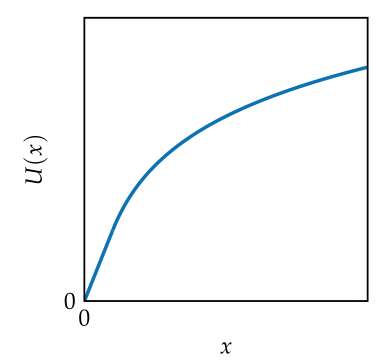
\includegraphics[scale=0.3]{figures/exponential_utility.png}
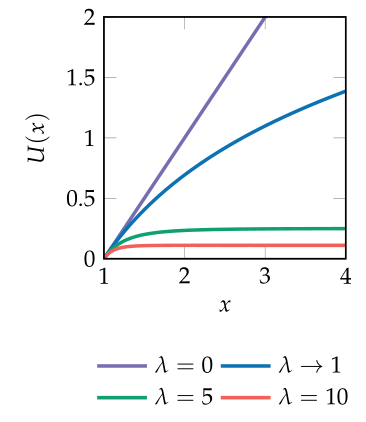
\includegraphics[scale=0.3]{figures/power_utility.png}
\end{frame}

\subsection{Power Utility = Risk Averse Proof}
\begin{frame}{Power Utility = Risk Averse Proof}
*see example notebook*
\end{frame}

\subsection{Maximum Expected Utility Principle}
\begin{frame}{Maximum Expected Utility Principle}
\begin{itemize}
    \item Maximum Expected Utility Principle := $EU(a|o) = \sum_{s'}P(s'|a,o)U(s')$
    \item Best action := $a^* = argmax_{a}EU(a|o)$
\end{itemize} 
\end{frame}

\section{Decision Networks}
\begin{frame}{Decision Networks}
Decision Network (sometimes called influence diagram) := a generalization of a Bayesian Network to include action and utility nodes so we may compactly represent the probability and utility models defining a decision problem. 

\subsection{Formulation}
Decision networks are composed of three types of nodes:
\begin{enumerate}[i]
    \item Chance Node := random variable
    \item Decision Node := Decision Variable
    \item Utility Node := Utility Node
\end{enumerate}
\end{frame}

\subsection{Edges}
\begin{frame}{Decision Network Edges}
Decision networks contain three kinds of directed edges:
\begin{enumerate}[i]
    \item Conditional Edge := edge which ends in a chance node and indicates the uncertainty in that chance conditioned on values of parents
    \item Informational Edge := edge which ends in a decision node and indicates that the decision associated with that node is made with knowledge of values of its parents 
    \item Functional Edge := edge which ends in a utility node and indicates that the utility node is determined by the outcomes of its parents
\end{enumerate}
\end{frame}

\subsection{Puppy Example}
\begin{frame}{Puppy Example}
*go to examples notebook*
    
\end{frame}


\section{Value of Information}
\begin{frame}{Value of Information}
\begin{itemize}
    \item Value of Information := utility of observing additional variables or observations.
    \item Expected utility of an optimal action given observation $o$ := $EU^*(o)$
    \item The value of information about variable $O'$ is given $o$ :=
    $VOI(O'|o) = (\sum_{o'} P(o'|o)EU^*(o,o')) - EU^*(o)$ 
\end{itemize}
\end{frame}

\end{document}
